 \section{Diagramme}
 
Zum Start des Projektes, hielt ich alle Ideen zum Projekt, in einer Requirements Tabelle fest. 
 
 \begin{figure}[htbp]
  \centering
     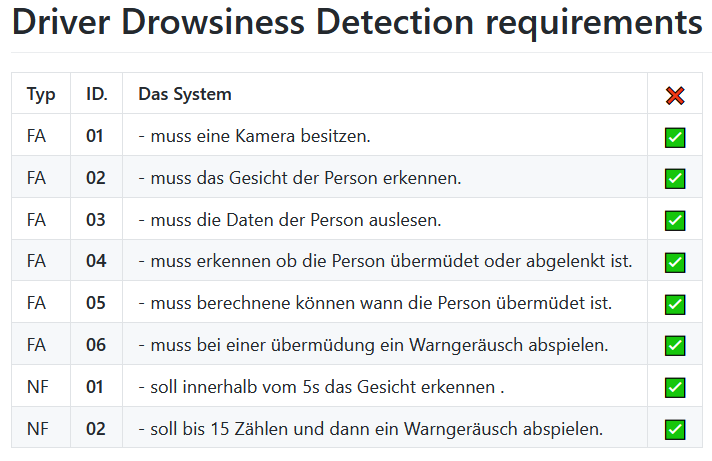
\includegraphics[width=0.48\textwidth]{DLReq.png}
     \caption{Requirements}
\end{figure}


Aus der Requirements Tabelle folgte ein Use-Case Diagramm, um den Ablauf der einzelnen Aktoren zu verdeutlichen.

\begin{figure}[htbp]
  \centering
     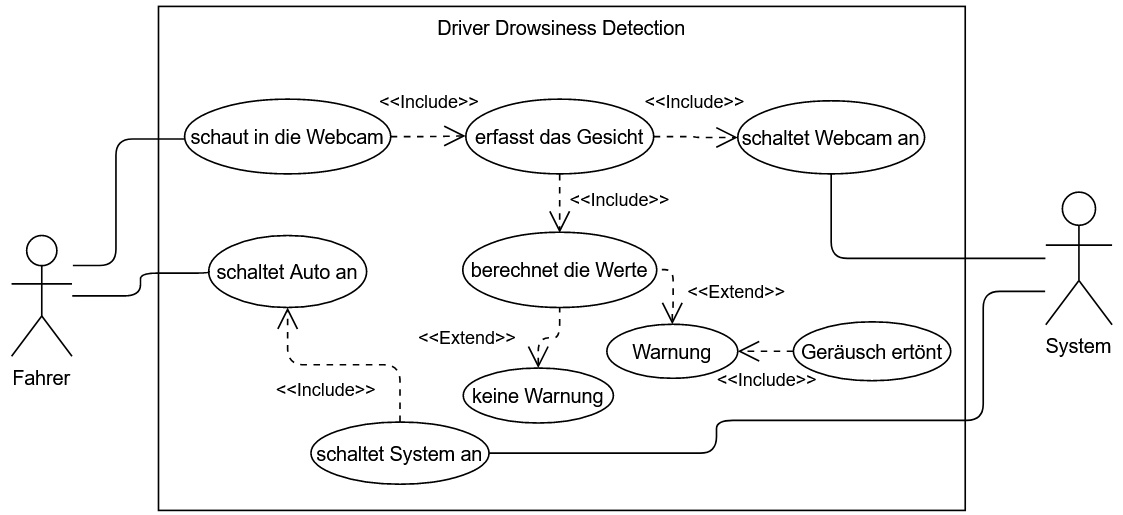
\includegraphics[width=0.48\textwidth]{UseCaseDL.png}
     \caption{Use-Case}
\end{figure}